\section{Results}
\label{xhw_study::sec::results}

\subsection{Sample Description}
\label{xhw_study::subsec::sample}
While participants' gender distribution is balanced, nearly 80\% of participants were between 18 and 44 years old and about 60\% had a post-secondary education.
The vast majority (92.4\%) of participants indicated that they had no practical experience designing, manufacturing, testing, or deploying hardware and were not involved with the subject at a policy level.
Participants exhibited a high degree of affinity for technology interaction ($M$$=$$4.05$, $SD$$=$$0.91$ on a 5-point scale).
\autoref{xhw_study::tab::demographics} in \autoref{xhw_study::app::demographics} provides detailed demographic information about the 250 participants.


\subsection{RQ1: End User Understanding of Microchips}
\label{xhw_study::subsec::coding_results}

\subsubsection{End-User Perception of Microchips}
\label{xhw_study::subsubsec::perceptions}
We coded participants' responses regarding their perceptions of microchips~(\autoref{xhw_study::question::perception}) as described in \autoref{xhw_study::subsec::analysis} and present the main results below.
See \autoref{xhw_study::tab::codebook_perception} in \autoref{xhw_study::app::codebook} for an overview of all assigned codes.

\paragraph{Participants' Perceptions Center Around Device Types} 
Participants primarily associate microchips with the applications they are deployed in. 
In 104 (42\%) cases, participants mentioned microchips' deployment in computers, followed by phones (47; 19\%), vehicles (22; 9\%), and tablets (8; 3\%). 
In addition to computers themselves, participants occasionally mentioned microchips' functioning as internal computer components (12; 5\%) or even more precisely, CPU (28; 11\%), motherboard (17; 7\%), and memory (13; 5\%). 
Participants also mentioned other devices or systems in 28 (11\%) cases such as robotics, credit cards, and household devices. 

Additionally, 71 (28\%) participants mentioned the broad notion that microchips are widespread and used across devices, using phrases such as \textit{\enquote{They are used in everything}} and \textit{\enquote{They power many things.}} 
Participants also associated microchips with technology (54; 22\%), electronics (50; 20\%), and technological advancement (47; 19\%), using phrases such as \textit{\enquote{they advance in technology constantly.}}

\paragraph{Microchip Shape and Composition}
Apart from the use cases of microchips, 84 (34\%) participants mentioned small size as a property of microchips (\eg, \textit{\enquote{Microchips are incredibly small}}). 
Another 35 (14\%) participants commented on the composition of microchips (\eg, \textit{\enquote{set of electronic circuits on a small piece}} and \textit{\enquote{silicon chips with thousands of [...] transistors}}). 
Furthermore, 22 (9\%) participants referred to the processing power of microchips (\eg, \textit{\enquote{powerhouse of the computer}} and \textit{\enquote{powerful processing system}}). 

\paragraph{Perceived Microchip Functionalities}
In 83 (33\%) cases, participants commented on microchips' general functionality as building blocks that make things work (\eg, \textit{\enquote{main components of personal computers}} and \textit{\enquote{make electronic devices work}}).
Some other participants delved into specific aspects of functionalities such as data storage (35; 14\%), data processing (25; 10\%), and communication capabilities (11; 4\%). 
Another 12 (5\%) participants described microchips as things that enact control (\eg, \textit{\enquote{dictate and command certain functions}}), and 15 (6\%) participants recognized microchips' diverse functionalities (\eg, \textit{\enquote{perform a variety of functions}}).

\paragraph{Misconceptions About Implanting Microchips}
A recurring theme among participants' responses was microchips being implanted into humans (29; 12\%) and animals (27; 11\%), conveyed in phrases such as \textit{\enquote{microchips being put into people}} and \textit{\enquote{inserted into dogs.}} 
This understanding likely comes from \enquote{microchipping} being a common term for animal implants in the United States.
Especially in the context of pets, tracking capabilities of microchips are mentioned in 18 (7\%) cases for \textit{\enquote{locating lost pets.}}
Microchips implanted into humans also co-occurred with conspiracy theories in 11 (4\%) cases.
In particular, six (2\%) participants mentioned microchips in the context of the COVID-19 pandemic (\eg, \textit{\enquote{We were all injected with one with the coronavirus vaccine}}).

\paragraph{Broader Societal and Security Implications Rarely Mentioned}
While microchips are featured prominently in geopolitical debates, supply chain issues about microchips were mentioned only occasionally in 18 (7\%) cases (\eg, \textit{\enquote{They are scarce in many places}} and \textit{\enquote{caused a massive shortage of vehicles}}). 
In particular, foreign manufacturing was identified as an issue in nine (4\%) cases (\eg, \textit{\enquote{Most that we need in America are made in Taiwan}}).
Another 20 (8\%) participants commented on microchips' societal impacts (\eg, \textit{\enquote{they are a major part of society}}) and political aspects (\eg, \textit{\enquote{they passed the CHIPS Act}}).
Only nine (4\%) participants mentioned security and privacy issues related to microchips proactively, commenting that microchips are \textit{\enquote{vulnerable to cybersecurity attacks}} and expressing \textit{\enquote{I have privacy concerns with them.}}

\subsubsection{End User Willingness to Understand More About Microchips}
\label{xhw_study::subsubsec::understand_more}
In \autoref{xhw_study::question::understand_more}, we asked participants whether they wanted to understand more about microchips and to provide reasons for their choice; we further asked participants about their aspirational and current time spent to understand microchips (\autoref{xhw_study::question::time_willing_before}) and ~(\autoref{xhw_study::question::time_actual}). \autoref{xhw_study::tab::codebook_understand} in \autoref{xhw_study::app::codebook} includes an overview of all assigned codes for participants' reasoning, and below we summarize key findings.

\paragraph{Participants Willing to Learn More About Microchips} 
In response to \autoref{xhw_study::question::understand_more}, 76\% of participants stated that they would like to know more about microchips, and 24\% did not want to know more.
When comparing responses to \autoref{xhw_study::question::time_willing_before} and \autoref{xhw_study::question::time_actual}, we observe the trend that participants would like to spend more time understanding microchips (\eg, for a newly acquired device) compared to the time they spend at the moment, reflecting a strong aspiration for learning more about microchips.
We asked participants twice about the time they are willing to spend on better understanding microchips---once at the beginning (\autoref{xhw_study::question::time_willing_before}) and once towards the end of the survey (\autoref{xhw_study::question::time_willing_after})---to check on potential social desirability bias, and we did not see noticeable changes in the responses to these two questions.

\paragraph{Motivation: Gaining Knowledge, as Existing Knowledge is Lacking}
In 96 (38\%) cases, participants mentioned that they want to know more about microchips to gain knowledge in general (\eg, \textit{\enquote{I like learning in general}} and \textit{\enquote{I can expand my knowledge}}). 
Another 20 (8\%) participants stated their motivation came from a desire of wanting to keep up with progress (\eg, \textit{\enquote{to stay up to date on technology}}), and 24 (10\%) expressed interest in following along the scientific progress (\eg, \textit{\enquote{I would love to know how it develops}}).
In addition, 46 (18\%) participants wanted to better understand the functionality of microchips (\eg, \textit{\enquote{I would like to know how they work}}), and 10 (4\%) wanted to better understand the manufacturing processes. 
The motivation to learn more is also related to participants' self-reported lack of existing knowledge, as 24 (10\%) participants stated that they had incomplete knowledge of microchips so far (\eg,\textit{\enquote{they feel a bit like magic}} and \textit{\enquote{I don't know much about them}}).


\paragraph{Motivation: Importance and Influence on (Future) Life}
In 32 (13\%) cases, participants acknowledged that microchips are omnipresent in daily life (\eg, \textit{\enquote{they became more integrated into our everyday lives}}). 
Additionally, 24 (10\%) participants mentioned microchips' impact on society (\eg, \textit{\enquote{what dangers it could bring to society}}) or their importance for the future (\eg, \textit{\enquote{it is a huge part of the future}}). 
Another 16 (6\%) participants commented that they wanted to broaden their understanding because of microchips' inherent link to technology (\eg, \textit{\enquote{I could learn how to better use tech}}). 

\paragraph{Hurdle: Lack of Interest and Need}
Among participants who did not want to know more about microchips, 28 (11\%) expressed that they have no interest in the topic (\eg, \textit{\enquote{I don't care}} and \textit{\enquote{It is a boring topic}}). 
Another 16 (6\%) participants did not see the need to understand more (\eg, \textit{\enquote{I know as much as I need to know about them}} and \textit{\enquote{It's not something I have to deal with a lot}}). 

\paragraph{Hurdle: Satisfaction, Complexity, and Fear}
In 25 (10\%) cases, participants mentioned that they were satisfied with their current level of knowledge about microchips or they would be satisfied as long as the microchips work as intended even if they do not know why (\eg, \textit{\enquote{as long as microchips work I don't care why or how}}). 
A total of 15 (6\%) participants felt that the topic was too complicated (\eg, \textit{\enquote{it sounds too intricate}} and \textit{\enquote{It's too complicated and will hurt my brain}}). 
Another eight (3\%) participants expressed fear regarding microchips in general (\eg,  \textit{\enquote{I worry what will be developed in the future}} and \textit{\enquote{I am afraid of them}}).

\begin{tcolorbox}
\subsubsection*{Summary in Light of RQ1}
\label{xhw_study::subsubsec::revisiting_rq1}
A majority of participants have a basic understanding of what microchips are, where they are deployed, and what they are capable of.
Furthermore, about three-quarters of our participants expressed a desire to learn more about microchips, mostly to expand their knowledge and keep up with the rapid technological advances.
Nevertheless, participants rarely commented on the societal implications of microchips or expressed concerns about the security and privacy aspects.
Thus, we observe that end users have the baseline knowledge and motivation to be involved as stakeholders in the hardware ecosystem, but educational efforts are needed to deepen their existing understanding and address misconceptions.
\end{tcolorbox}

\subsection{RQ2: Importance of Desiderata and Information Types}
\label{xhw_study::subsec::descriptive}

\subsubsection{Criticality of Microchip Application Settings}
\label{xhw_study::subsubsec::setting_criticality}
\autoref{xhw_study::fig::criticality_settings} depicts our participants' perceived criticality of the five settings on a scale from \textit{1---not at all critical} to \textit{5---extremely critical}.
In line with our expectations, the most critical settings were microchips deployed in an airplane ($M$$=$$4.72$, $SD$$=$$0.69$) and in a pacemaker ($M$$=$$4.71$, $SD$$=$$0.83$).
The two settings at the intermediate level were microchips that enable wireless communication in a cell tower ($M$$=$$3.86$, $SD$$=$$1.04$) and microchips that enable fingerprint unlocking in a smartphone ($M$$=$$3.20$, $SD$$=$$1.20$).
Microchips in the entertainment system of a car were rated the least critical ($M$$=$$2.66$, $SD$$=$$1.28$). 

\pgfplotstableread{
Label       t1 t2 t3 t4 t5
heartbeat~in~pacemaker   7 2 12 15 214
steering~of~airplane    1 5 14 22 208
wireless~communication~of~cell~tower  7 18 59 84 82
fingerprint~unlocking~in~smartphone  24 48 73 65 40
entertainment~system~in~car         55 66 69 29 31
}\critdata

\begin{figure*}[htbp]
    \footnotesize
    \centering
    \begin{tikzpicture}
        \begin{axis}[
            xbar stacked, 
            xmin=0,
            y=10pt,
            bar width=5pt,
            ytick=data, 
            yticklabels from table={\critdata}{Label},
            enlarge y limits={abs=5pt},
            enlarge x limits={abs=5pt},
            axis y line*=left,
            axis x line*=bottom,
            xtick align=outside,
            ytick align=inside,
            legend columns=1,
            legend pos=outer north east,
            legend cell align=left,
        ]
            \addplot [fill=c1] table [x=t1, meta=Label,y expr=\coordindex] {\critdata};
            \addplot [fill=c2] table [x=t2, meta=Label,y expr=\coordindex] {\critdata};
            \addplot [fill=c3] table [x=t3, meta=Label,y expr=\coordindex] {\critdata};
            \addplot [fill=c4] table [x=t4, meta=Label,y expr=\coordindex] {\critdata};
            \addplot [fill=c5] table [x=t5, meta=Label,y expr=\coordindex] {\critdata};
            \legend{1---not at all critical,2---slightly critical,3---moderately critical,4---very critical,5---extremely critical}
        \end{axis}
    \end{tikzpicture}
    \caption{Participants' criticality ratings of the five different settings presented in our survey vignettes.}
    \label{xhw_study::fig::criticality_settings}
    \Description{The figure depicts a horizontal stacked bar chart comprising five bars of five sections each and a legend to the right of the bar chart. On the x-axis, all bars span from 0 to 250. On the y-axis, the first bar (the top one) is labeled "entertainment system in car", the second bar is labeled "fingerprint unlocking in smartphone", the third bar is labeled "wireless communication of cell tower", the fourth bar is labeled "steering of airplane", the fifth (and last) bar is labeled "heartbeat in pacemaker". The legend on the right then assigns meanings to the segments of each bar. It comprises five labels and is organized in two columns of three rows that are to be read from top to bottom first, left to right second. The first label says "1-not at all critical", the second "2-slightly critical", the third "3-moderately critical", the fourth "4-very critical", and the fifth "5-extremely critical".}
\end{figure*}

A Welch's ANOVA revealed significant differences in the perceived criticality across scenarios ($F(4)$$=$$198.35$, $p$$<$$.001$).
Subsequent pairwise Wilcoxon rank sum tests with Bonferroni corrections revealed significant differences between all scenarios except between the airplane and pacemaker scenarios.

\begin{figure}[htb]
    \centering
    \footnotesize
    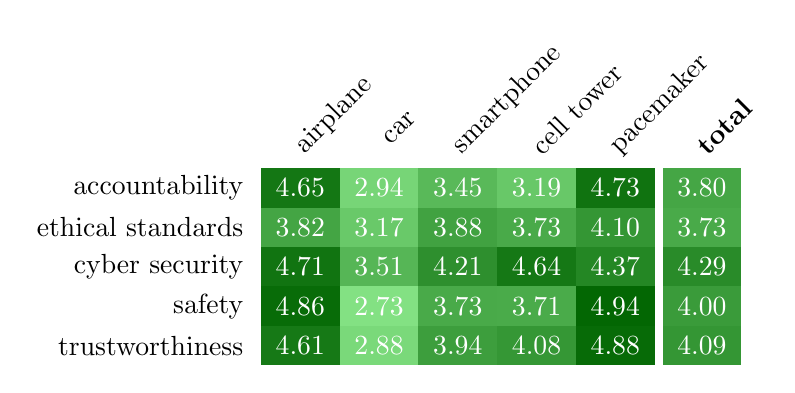
\begin{tikzpicture}[scale=1]
        \foreach \y [count=\n] in {
            {4.65,2.94,3.45,3.19,4.73,3.80},
            {3.82,3.17,3.88,3.73,4.10,3.73},
            {4.71,3.51,4.21,4.64,4.37,4.29},
            {4.86,2.73,3.73,3.71,4.94,4.00},
            {4.61,2.88,3.94,4.08,4.88,4.09},
        } {
            \foreach \x [count=\m] in \y {
                \pgfmathsetmacro{\scaledx}{100 - (\x - 2.5) * 40}
                \pgfmathsetmacro{\xpos}{\m + (\m==6 ? 0.1 : 0)}
                \pgfmathsetmacro{\ypos}{-\n*0.5 - 0.2}
                \ifnum\n=6\else
                    \node[fill=LightGreen!\scaledx!DarkGreen, minimum height=5mm,minimum width=10mm, text=white] at (\xpos,\ypos) {\x};
                \fi
            }
        }
    
        % row labels
        \foreach \a [count=\i] in {airplane,car,smartphone,cell tower,pacemaker,\textbf{total}} {
            \pgfmathsetmacro{\xpos}{\i + (\i==6 ? 0.1 : 0)}
            \node[minimum height=5mm,minimum width=10mm,left,right,rotate=45] at (\xpos-0.1, -0.3) {\a};
        }
    
        % column labels
        \foreach \a [count=\i] in {accountability,ethical standards,cyber security,safety, trustworthiness} {
            \pgfmathsetmacro{\ypos}{-\i*0.5 - 0.2}
            \node[minimum height=5mm,minimum width=10mm,left] at (0.4,\ypos) {\a};
        }
    \end{tikzpicture}
    \caption{Participants' mean importance ratings of our desiderata in the context of the considered settings.}
    \label{xhw_study::fig::importance_desiderata}
    \Description{The figure shows a six-by-five heatmap comprising decimal numbers between 1 (lowest) and 5 (highest) for each entry in the six-by-five grid. On the x-axis, the settings "airplane", "car", "smartphone", "cell tower", and "pacemaker" are displayed together with an additional column labeled "total" that is separated from the heatmap by some whitespace. On the y-axis, the five desiderata "accountability", "ethical standards", "cyber security", "safety", and "trustworthiness" are given. The heat map entries are colored in different shades of blue depending on their value. The higher the value, the darker the blue color.}
\end{figure}

\subsubsection{Importance of Desiderata in Different Settings}
\label{xhw_study::subsubsec::desiderata_importance}
We asked participants about their perceived importance of five desiderata on a scale from \textit{1---not at all important} to \textit{5---extremely important}. 
The most important desiderata were cyber security ($M$$=$$4.29$, $SD$$=$$1.11$) and trustworthiness ($M$$=$$4.09$, $SD$$=$$1.19$). 
Safety comes in third ($M$$=$ $4.00$, $SD$$=$$1.31$) followed by accountability ($M$$=$$3.80$, $SD$$=$$1.35$) and ethical standards ($M$$=$$3.73$, $SD$$=$$1.28$).
\autoref{xhw_study::fig::importance_desiderata} reports more fine-grained mean values, connecting each desideratum to the different microchip application settings.

\subsubsection{Importance of Information Types}
We asked participants to rate the importance of different types of information in relation to the deployment setting and desideratum respectively, on a scale from \textit{1---not at all important} to \textit{5---extremely important}. 
Across all desiderata and settings, information on \textit{which functionality} a microchip provides was rated the most important ($M$$=$$3.60$, $SD$$=$$1.33$).
This is followed by information about how a microchip was \textit{approved for use} ($M$$=$$3.56$, $SD$$=$$1.36$) and how the microchip \textit{interacts with the surrounding system} ($M$$=$$3.51$, $SD$$=$$1.38$).
Participants placed less importance on the manufacturing aspects, namely information on \textit{who manufactured} the microchip ($M$$=$$3.32$, $SD$$=$$1.38$) 
and information on \textit{how a microchip was manufactured} ($M$$=$$3.25$, $SD$$=$$1.35$).

\pgfplotstableread{
Label                t1 t2 t3 t4 t5
who~manufactured     26 29 52 55 88
how~interacts        23 22 44 59 102
how~approved         19 22 38 59 112
which~functionality  20 29 39 61 101
how~manufactured     23 37 57 52 81
}\infsetairplane

\pgfplotstableread{
Label                t1 t2 t3 t4 t5
who~manufactured     49 55 64 43 39
how~interacts        48 42 56 54 50
how~approved         50 48 51 48 53
which~functionality  36 39 69 48 58
how~manufactured     53 58 57 47 35
}\infsetcar

\pgfplotstableread{
Label                t1 t2 t3 t4 t5
who~manufactured     38 35 61 60 56
how~interacts        36 32 56 59 67
how~approved         33 32 58 62 65
which~functionality  32 29 56 56 77
how~manufactured     45 39 69 50 47
}\infsetsmartphone

\pgfplotstableread{
Label                t1 t2 t3 t4 t5
who~manufactured     44 42 60 50 54
how~interacts        38 37 55 57 63
how~approved         31 36 57 64 62
which~functionality  34 29 58 70 59
how~manufactured     35 54 73 43 45
}\infsetcelltower

\pgfplotstableread{
Label                t1 t2 t3 t4 t5
who~manufactured     20 25 38 73 94
how~interacts        15 12 37 66 120
how~approved         12 12 30 66 130
which~functionality  9 12 34 64 131
how~manufactured     14 25 45 71 95
}\infsetpacemaker

\begin{figure*}[htbp]
    \centering
    \begin{tikzpicture}
        \begin{groupplot}[group style={group size=2 by 3, horizontal sep=2.4cm, vertical sep=0.9cm},
        /pgfplots/legend style={at={(0.5,4.6)}, anchor=north, legend columns=5}]
            \pgfplotsset{my bar/.style={width=6cm,
                xbar stacked, ymin=0,  
                xmin=0,
                y=10pt,
                bar width=5pt,
                ytick=data, 
                yticklabels from table={\infsetairplane}{Label},
                enlarge y limits={abs=5pt},
                axis y line*=left,
                axis x line*=bottom,
                xtick align=outside,
                ytick align=inside,
                font=\footnotesize,
                enlarge x limits={abs=5pt},
                title style={yshift=-0.25cm}
                }}
            \nextgroupplot[my bar, title=\textbf{steering of airplane}]
                \addplot [fill=c1] table [x=t1, meta=Label,y expr=\coordindex] {\infsetairplane};
                \addplot [fill=c2] table [x=t2, meta=Label,y expr=\coordindex] {\infsetairplane};
                \addplot [fill=c3] table [x=t3, meta=Label,y expr=\coordindex] {\infsetairplane};
                \addplot [fill=c4] table [x=t4, meta=Label,y expr=\coordindex] {\infsetairplane};
                \addplot [fill=c5] table [x=t5, meta=Label,y expr=\coordindex] {\infsetairplane};
            \nextgroupplot[my bar, title=\textbf{entertainment system in car}]
                \addplot [fill=c1] table [x=t1, meta=Label,y expr=\coordindex] {\infsetcar};
                \addplot [fill=c2] table [x=t2, meta=Label,y expr=\coordindex] {\infsetcar};
                \addplot [fill=c3] table [x=t3, meta=Label,y expr=\coordindex] {\infsetcar};
                \addplot [fill=c4] table [x=t4, meta=Label,y expr=\coordindex] {\infsetcar};
                \addplot [fill=c5] table [x=t5, meta=Label,y expr=\coordindex] {\infsetcar};
            \nextgroupplot[my bar, title=\textbf{fingerprint unlocking in smartphone}]
                \addplot [fill=c1] table [x=t1, meta=Label,y expr=\coordindex] {\infsetsmartphone};
                \addplot [fill=c2] table [x=t2, meta=Label,y expr=\coordindex] {\infsetsmartphone};
                \addplot [fill=c3] table [x=t3, meta=Label,y expr=\coordindex] {\infsetsmartphone};
                \addplot [fill=c4] table [x=t4, meta=Label,y expr=\coordindex] {\infsetsmartphone};
                \addplot [fill=c5] table [x=t5, meta=Label,y expr=\coordindex] {\infsetsmartphone};
            \nextgroupplot[my bar, title=\textbf{wireless communication of cell tower}]
                \addplot [fill=c1] table [x=t1, meta=Label,y expr=\coordindex] {\infsetcelltower};
                \addplot [fill=c2] table [x=t2, meta=Label,y expr=\coordindex] {\infsetcelltower};
                \addplot [fill=c3] table [x=t3, meta=Label,y expr=\coordindex] {\infsetcelltower};
                \addplot [fill=c4] table [x=t4, meta=Label,y expr=\coordindex] {\infsetcelltower};
                \addplot [fill=c5] table [x=t5, meta=Label,y expr=\coordindex] {\infsetcelltower};
            \nextgroupplot[my bar, title=\textbf{heartbeat in pacemaker}, at = {($($(group c1r2.south west) + (0,-1.8cm)$ )!0.5!(group c2r2.south east)$) }]
                \addplot [fill=c1] table [x=t1, meta=Label,y expr=\coordindex] {\infsetpacemaker};
                \addplot [fill=c2] table [x=t2, meta=Label,y expr=\coordindex] {\infsetpacemaker};
                \addplot [fill=c3] table [x=t3, meta=Label,y expr=\coordindex] {\infsetpacemaker};
                \addplot [fill=c4] table [x=t4, meta=Label,y expr=\coordindex] {\infsetpacemaker};
                \addplot [fill=c5] table [x=t5, meta=Label,y expr=\coordindex] {\infsetpacemaker};
        \legend{1---not at all important,2---slightly important,3---moderately important,4---very important,5---extremely important}
        \end{groupplot}
     \end{tikzpicture}
    \caption{Importance of different types of information depending on the setting in which microchips are employed. The results are aggregated across all desiderata.}
    \label{xhw_study::fig::importance_information_settings}
    \Description{The figure shows five horizontal bar charts, every one of them comprising a title and five bars of five sections each. The bar charts are arranged in a V-shape: two on top, two in the middle, and a last one centered below the middle two. All bar charts share a common legend among them, which is placed on top of them all. The labels of each bar chart are the same apart from their title. From left to right, top to bottom, the bar chart titles read "steering of airplane", "entertainment system in car", "fingerprint unlocking in smartphone", "wireless communication of cell tower", and "heartbeat in pacemaker". On the x-axis of each chart, all bars span from 0 to 250. On the y-axis of each chart, the first bar (the top one) is labeled "how manufactured", the second bar is labeled "which functionality", the third bar is labeled "how approved", the fourth bar is labeled "how interacts", the fifth (and last) bar is labeled "who manufactured". The legend on at the top then assigns meanings to the segments of each bar. It comprises five labels and is organized in a single row. The first label says "1-not at all important", the second "2-slightly important", the third "3-moderately important", the fourth "4-very important", and the fifth "5-extremely important".}
\end{figure*}


\pgfplotstableread{
Label                t1 t2 t3 t4 t5
who~manufactured     43 36 69 49 53
how~interacts        32 30 53 63 72
how~approved         29 26 45 62 88
which~functionality  24 36 51 58 81
how~manufactured     38 44 71 41 56
}\infdessafety

\pgfplotstableread{
Label                t1 t2 t3 t4 t5
who~manufactured     31 43 43 51 82
how~interacts        32 33 46 56 83
how~approved         28 36 52 60 74
which~functionality  27 25 65 53 80
how~manufactured     34 47 57 52 60
}\infdesaccountability

\pgfplotstableread{
Label                t1 t2 t3 t4 t5
who~manufactured     31 29 54 63 73
how~interacts        46 34 50 50 70
how~approved         34 31 47 59 79
which~functionality  40 29 48 59 74
how~manufactured     28 36 52 58 76
}\infdesethical

\pgfplotstableread{
Label                t1 t2 t3 t4 t5
who~manufactured     32 35 56 62 65
how~interacts        23 18 43 67 99
how~approved         22 26 42 62 98
which~functionality  18 27 39 67 99
how~manufactured     34 43 57 60 56
}\infdessecurity

\pgfplotstableread{
Label                t1 t2 t3 t4 t5
who~manufactured     40 43 53 56 58
how~interacts        27 30 56 59 78
how~approved         32 31 48 56 83
which~functionality  22 21 53 62 92
how~manufactured     36 43 64 52 55
}\infdestrustworthiness

\begin{figure*}[htbp]
    \centering
    \begin{tikzpicture}
        \begin{groupplot}[group style={group size=2 by 3, horizontal sep=2.4cm, vertical sep=0.9cm},
        /pgfplots/legend style={at={(0.5,4.6)}, anchor=north, legend columns=5}]
            \pgfplotsset{my bar/.style={width=6cm,
                xbar stacked, ymin=0,  
                xmin=0,
                y=10pt,
                bar width=5pt,
                ytick=data, 
                yticklabels from table={\infdessafety}{Label},
                enlarge y limits={abs=5pt},
                axis y line*=left,
                axis x line*=bottom,
                xtick align=outside,
                ytick align=inside,
                font=\footnotesize,
                enlarge x limits={abs=5pt},
                title style={yshift=-0.25cm}
                }}
            \nextgroupplot[my bar, title=\textbf{safety}]
                \addplot [fill=c1] table [x=t1, meta=Label,y expr=\coordindex] {\infdessafety};
                \addplot [fill=c2] table [x=t2, meta=Label,y expr=\coordindex] {\infdessafety};
                \addplot [fill=c3] table [x=t3, meta=Label,y expr=\coordindex] {\infdessafety};
                \addplot [fill=c4] table [x=t4, meta=Label,y expr=\coordindex] {\infdessafety};
                \addplot [fill=c5] table [x=t5, meta=Label,y expr=\coordindex] {\infdessafety};
            \nextgroupplot[my bar, title=\textbf{accountability}]
                \addplot [fill=c1] table [x=t1, meta=Label,y expr=\coordindex] {\infdesaccountability};
                \addplot [fill=c2] table [x=t2, meta=Label,y expr=\coordindex] {\infdesaccountability};
                \addplot [fill=c3] table [x=t3, meta=Label,y expr=\coordindex] {\infdesaccountability};
                \addplot [fill=c4] table [x=t4, meta=Label,y expr=\coordindex] {\infdesaccountability};
                \addplot [fill=c5] table [x=t5, meta=Label,y expr=\coordindex] {\infdesaccountability};
            \nextgroupplot[my bar, title=\textbf{ethical standards}]
                \addplot [fill=c1] table [x=t1, meta=Label,y expr=\coordindex] {\infdesethical};
                \addplot [fill=c2] table [x=t2, meta=Label,y expr=\coordindex] {\infdesethical};
                \addplot [fill=c3] table [x=t3, meta=Label,y expr=\coordindex] {\infdesethical};
                \addplot [fill=c4] table [x=t4, meta=Label,y expr=\coordindex] {\infdesethical};
                \addplot [fill=c5] table [x=t5, meta=Label,y expr=\coordindex] {\infdesethical};
            \nextgroupplot[my bar, title=\textbf{cyber security}]
                \addplot [fill=c1] table [x=t1, meta=Label,y expr=\coordindex] {\infdessecurity};
                \addplot [fill=c2] table [x=t2, meta=Label,y expr=\coordindex] {\infdessecurity};
                \addplot [fill=c3] table [x=t3, meta=Label,y expr=\coordindex] {\infdessecurity};
                \addplot [fill=c4] table [x=t4, meta=Label,y expr=\coordindex] {\infdessecurity};
                \addplot [fill=c5] table [x=t5, meta=Label,y expr=\coordindex] {\infdessecurity};
            \nextgroupplot[my bar, title=\textbf{trustworthiness}, at = {($($(group c1r2.south west) + (0,-1.8cm)$ )!0.5!(group c2r2.south east)$) }]
                \addplot [fill=c1] table [x=t1, meta=Label,y expr=\coordindex] {\infdestrustworthiness};
                \addplot [fill=c2] table [x=t2, meta=Label,y expr=\coordindex] {\infdestrustworthiness};
                \addplot [fill=c3] table [x=t3, meta=Label,y expr=\coordindex] {\infdestrustworthiness};
                \addplot [fill=c4] table [x=t4, meta=Label,y expr=\coordindex] {\infdestrustworthiness};
                \addplot [fill=c5] table [x=t5, meta=Label,y expr=\coordindex] {\infdestrustworthiness};
        \legend{1---not at all important,2---slightly important,3---moderately important,4---very important,5---extremely important}
        \end{groupplot}
     \end{tikzpicture}
    \caption{Importance of different kinds of information depending on the desiderata to be evaluated by the end user. The results are aggregated across all settings.}
    \label{xhw_study::fig::importance_information_desiderata}
    \Description{The figure shows five horizontal bar charts, every one of them comprising a title and five bars of five sections each. The bar charts are arranged in a V-shape: two on top, two in the middle, and a last one centered below the middle two. All bar charts share a common legend among them, which is placed on top of them all. The labels of each bar chart are the same apart from their title. From left to right, top to bottom, the bar chart titles read "safety", "accountability", "ethical standards", "cyber security", and "trustworthiness". On the x-axis of each chart, all bars span from 0 to 250. On the y-axis of each chart, the first bar (the top one) is labeled "how manufactured", the second bar is labeled "which functionality", the third bar is labeled "how approved", the fourth bar is labeled "how interacts", the fifth (and last) bar is labeled "who manufactured". The legend on at the top then assigns meanings to the segments of each bar. It comprises five labels and is organized in a single row. The first label says "1-not at all important", the second "2-slightly important", the third "3-moderately important", the fourth "4-very important", and the fifth "5-extremely important".}
\end{figure*}


\autoref{xhw_study::fig::importance_information_settings} shows the trend that the type of information desired by end users depends on the application setting in which they are used at least to some extent. Information on the functionality of a microchip, how it has been approved for use, and how it interacts with the system were perceived to be more important than the other types of information, particularly in airplane and pacemaker settings.
For other settings, such as the car and the smartphone, these differences still exist but are not as pronounced. For instance, information on a microchip's functionality was rated the most important for the smartphone setting.

\autoref{xhw_study::fig::importance_information_desiderata} shows that the desired information types may also depend on the target desideratum.
For example, to evaluate cyber security and trustworthiness, information on the microchip's functionality, how it has been approved for use, and how it interacts with the system were rated more important than the manufacturing-related information.
A similar trend was observed for safety, although here, information on how the microchips have been approved has a small edge over the two others.
When end users want to evaluate accountability or ethical standards, the ratings were similar and no particular types of information stood out.

\begin{tcolorbox}
\subsubsection*{Summary in Light of RQ2} 
Participants had diverse perceptions regarding the criticality of different application settings for microchips. 
While participants considered all five desiderata very important ($M$$>$$3.5$ for all), cyber security and trustworthiness emerged to be the more important ones.
For information types, participants desired to know more about the microchip's functionality, how it is approved for use, and how it interacts with the underlying system than about the manufacturing processes. 
We also observe the trend that the desired information types depend on the application setting and the target desideratum, and we quantitatively test the correlations in~\autoref{xhw_study::subsec::regression_information}.
\end{tcolorbox}

\subsection{RQ3: Factors Shaping End Users' Information Needs}
\label{xhw_study::subsec::regression_information}

To gain more granular insight into the factors that shape end users' information needs, we applied multilevel regression modeling to each of the five information types.
For settings, the \textit{microchips controlling the entertainment system in a car} was used as a baseline because of its lowest criticality rating (see~\autoref{xhw_study::subsubsec::setting_criticality}).
For desiderata, \textit{ethical standards} was chosen as the baseline as participants rated it as least important (see \autoref{xhw_study::subsubsec::desiderata_importance}).
Compared to the intercept-only models without any predictors, the random intercept models containing the settings and desiderata had significantly lower deviances (\eg, $\chi^2(8)$$=$$59.95$, $p$$<$$.001$ for the \textit{which functionality} model), indicating a better fit to our data.

\begin{table*}[htbp]
    \centering
    \footnotesize
    \caption{Multilevel regression analysis based on participants' ratings of the importance of receiving different types of information to evaluate a desideratum in a given setting, on a scale from \textit{1---not at all important} to \textit{5---extremely important}.}% (see \autoref{xhw_study::question::v0_information} for an example question presented to participants).}
    \label{xhw_study::tab::regression_information}
    \begin{tabularx}{\textwidth}{XL{1.5cm}L{1.5cm}L{1.5cm}L{1.5cm}L{1.5cm}}
        \toprule
         & \textbf{which func-} & \textbf{how} & \textbf{how} & \textbf{who manu-} &  \textbf{how manu-} \\
         & \textbf{tionality} &  \textbf{interacts} & \textbf{approved}  & \textbf{factured}  & \textbf{factured}\\
         \textit{Predictors} & \textit{Est.} & \textit{Est.} & \textit{Est.} &  \textit{Est.} & \textit{Est.} \\
         \midrule
        intercept: ethical standards (desideratum) $\times$ car (setting) & \textbf{2.61***} & \textbf{2.35***} & \textbf{2.63***} & \textbf{2.66***}  & \textbf{2.71***} \\
        \midrule
         \textit{setting (baseline=car)} & & & & & \\
        smartphone & 0.25 %**
        & 0.29
        %**
        & \textbf{0.35***} &  0.25 %**
        & \textbf{0.37***} \\
        cell tower & 0.15 & 0.21 %*
        & \textbf{0.34***} & 0.22 %**
        & 0.24 
        %**
        \\
        pacemaker & \textbf{0.97***} & \textbf{0.99***} &  \textbf{1.13***} & \textbf{1.02***} & \textbf{0.92***} \\
        airplane & \textbf{0.56***} & \textbf{0.71***} &  \textbf{0.87***} & \textbf{0.72***} & \textbf{0.73***} \\
        \midrule
        \textit{desideratum (baseline=ethical standards)} & & & & & \\
        accountability & 0.13 & 0.23 %*
        & -0.02 & -0.25 %**  
        & -0.04 \\
        safety & 0.14 & 0.18 %*
        & 0.13 &  \textbf{-0.36***} & \textbf{-0.35***} \\
        trustworthiness & \textbf{0.32***} & 0.25 %**
        & 0.02 & \textbf{-0.30***} & -0.29 %**
        \\
        cyber security & \textbf{0.41***} & \textbf{0.54***} &  0.27 %** 
        & -0.24 %** 
        & -0.11 \\
        \midrule
        desire to understand more about microchips & \textbf{0.53***} & \textbf{0.63***} & 0.41 %**
        & 0.50 %**
        & 0.43 %* 
        \\
        ATI score & \textbf{0.26***} & \textbf{0.27***} & 0.23 %**
        & 0.26 %**
        & 0.24 %**
        \\
        % \midrule
        \midrule
        marginal $R^2$    & 0.171 & 0.190 & 0.155 & 0.165 & 0.129\\
        conditional $R^2$ & 0.461 & 0.469 & 0.507 & 0.554 & 0.521\\    
        \bottomrule
     \end{tabularx}
     \textit{
     % * p < 0.05; ** p < 0.01, 
     *** $p$$<$$.001$; we only highlighted coefficients with $p$$<$$.001$ due to the Bonferroni correction}
     \label{xhw_study::subsec::regression_results}
     \Description{The table is organized in six columns. In the first column on the left, the predictors for multilevel regression analysis are given. Each of the other five major columns provides details on a type of information about microchips, starting with "which functionality" on the left and ending with "how manufactured" on the right. Each row of the five major columns gives the Estimate ("Est.") for one predictor. Here, "***" following an estimate means p<0.001, and respective entries are highlighted in boldface. In the first line below the table headers, the intercept of regression analysis is given for each kind of information. Next, a sub-header spanning the entire table titled "settings (baseline=car)" opens the section with the analysis results for the four settings "smartphone", "cell tower", "pacemaker", and "airplane". The estimates for these settings are given in the next 4 rows. Next, a sub-header spanning the entire table titled "Desiderata (baseline=ethical standards)" opens the section with the analysis results for the four desiderata "accountability", "safety", "trustworthiness", and "cyber security". The estimates for these desiderata are given in the next 4 rows. In the next section, the first row is titled "desire to understand more about microchips" and lists respective estimates. The second and final row of this section is titled "ATI score" and lists respective estimates. Finally, in the last section of the table, the first row lists results for "marginal R^2" and the second row "conditional R^2".}
\end{table*}

We then tested the specific predictors for the significant explanatory power expressed by marginal $R^2$.
In addition to the application setting's perceived criticality and the desideratum's perceived importance as the main effects, we included participants' general desire to understand more about microchips as a binary predictor (\textit{no} as the baseline) and their \ac{ATI} score~\cite{franke2019personal} (applying grand-mean centering, utilizing the \ac{ATI} mean value as the baseline).
We further tried including participants' demographics (\ie, gender, age, and educational background) in our models, but they did not add significantly more explanatory power.
We thus omit these variables from the analysis.
Our final models with the random intercept reached a better fit ($\ac{AIC}$$=$$[3725.2 - 3913.7]$;  $\ac{BIC}$$=$$[3806.9 - 4062.5]$) compared to our base models ($\ac{AIC}$$=$$[3969.6 - 4123.4]$;  $\ac{BIC}$$=$$[3985.0 - 4138.8]$).

\autoref{xhw_study::subsec::regression_results} shows the regression outputs. 
Below we unpack a few key findings. 
We report separate regression models that look into the interaction effects between settings and desiderata in \autoref{xhw_study::app::regression_results}, which show similar patterns as the findings reported here.\footnote{While the models with interaction effects enable a more nuanced examination of information needs in response to individual vignettes, the number of participants per vignette was limited to 25, negatively affecting the statistical power and increasing the alpha error accumulation. 
We thus opted to report the interaction effects in \autoref{xhw_study::app::regression_results}.}



\paragraph{Higher Information Needs for Critical Settings} 
Looking at the main effect of application settings, we observe that settings with higher criticality ratings were significantly correlated with higher information needs. 
Compared to \textit{car} as the baseline, participants gave significantly higher ratings across the five information types for vignettes featuring \textit{airplane} and \textit{pacemaker}. 
\textit{Smartphone} and \textit{cell tower} as setting also drove up the information needs to some degree. 
However, this pattern only applies to certain types of information, namely \textit{how the microchip is approved for use} (for both settings) and \textit{how the microchip is manufactured} (only for \textit{smartphone}).

\paragraph{Nuanced Influences from Desiderata}
In contrast to findings on application settings, where there was a clear association between high perceived criticality and high information needs, the effect of desiderata on information needs is more nuanced.
Compared to ethical standards, participants had a stronger desire for information on the microchip's functionality and how it interacts with the system when \textit{cyber security} was the target desideratum. 
Participants also valued information on the microchip's functionality for \textit{trustworthiness}. 
Conversely, participants attached less importance to information about the microchip's manufacturing process, but only when the target desiderata were \textit{safety} (for both information types) and \textit{trustworthiness} (for \textit{who manufactured} only).
Between ethical standards and \textit{accountability}, participants' information needs were similar with no statistically significant differences.

\paragraph{Information Needs Shaped by the Desire to Understand and \acs{ATI}}
A general desire of participants to know more about microchips also shapes participants' information needs. 
The coefficients are positive across the five information types, and the influences were particularly pronounced for information on the microchip's functionality and how the microchip interacts with the system.
These observations are in line with our findings regarding RQ1, where participants shared their willingness to learn more about microchips open-endedly, and their existing understandings revolve around functionalities and application settings.
Similarly, a higher \ac{ATI} score contributes to more desire for information, particularly for functionality and interactions with the system. 

\begin{tcolorbox}
\subsubsection*{Summary in Light of RQ3.}
The factors driving end users' information needs are multifaceted. 
Higher information needs generally occurred when participants perceived the setting in which the microchip was deployed to be highly critical, whereas desiderata do not consistently predict information needs. 
Participants' general desire to understand microchips and \ac{ATI} also played a significant role in shaping information needs, particularly for the microchip's functionality and how it interacts with the system.
\end{tcolorbox}